\documentclass{article}
\usepackage[T1]{fontenc}
\usepackage{lmodern}
\usepackage{graphicx}
\usepackage{amsmath,amssymb}
\usepackage[a4paper,margin=2cm]{geometry}
\usepackage[absolute,overlay]{textpos}
\setlength{\TPHorizModule}{1mm}
\setlength{\TPVertModule}{1mm}
\usepackage[indonesian]{babel}
\usepackage{hyperref}
\setlength{\emergencystretch}{2em}
% unit: Halaman 3

\begin{document}

% === Halaman 3 (llm) ===

\vspace{198.99mm}

\textcolor{red}{Blok plainteks berukuran $n$ bit:}
\[ P = (p_1, p_2, ..., p_n), p_i \in \{0, 1\} \]
\vspace{5mm}
\textcolor{red}{Blok cipherteks berukuran $n$ bit:}
\[ C = (c_1, c_2, ..., c_n), c_i \in \{0, 1\} \]

% deskripsi: Diagram proses enkripsi yang menunjukkan Blok plainteks P dan Kunci K masuk ke fungsi Enkripsi E untuk menghasilkan Blok cipherteks C.
% bbox normalisasi: [0.0600, 0.1080, 0.9400, 0.9120]
\begin{textblock*}{184.80mm}(12.60mm,32.08mm)
\noindent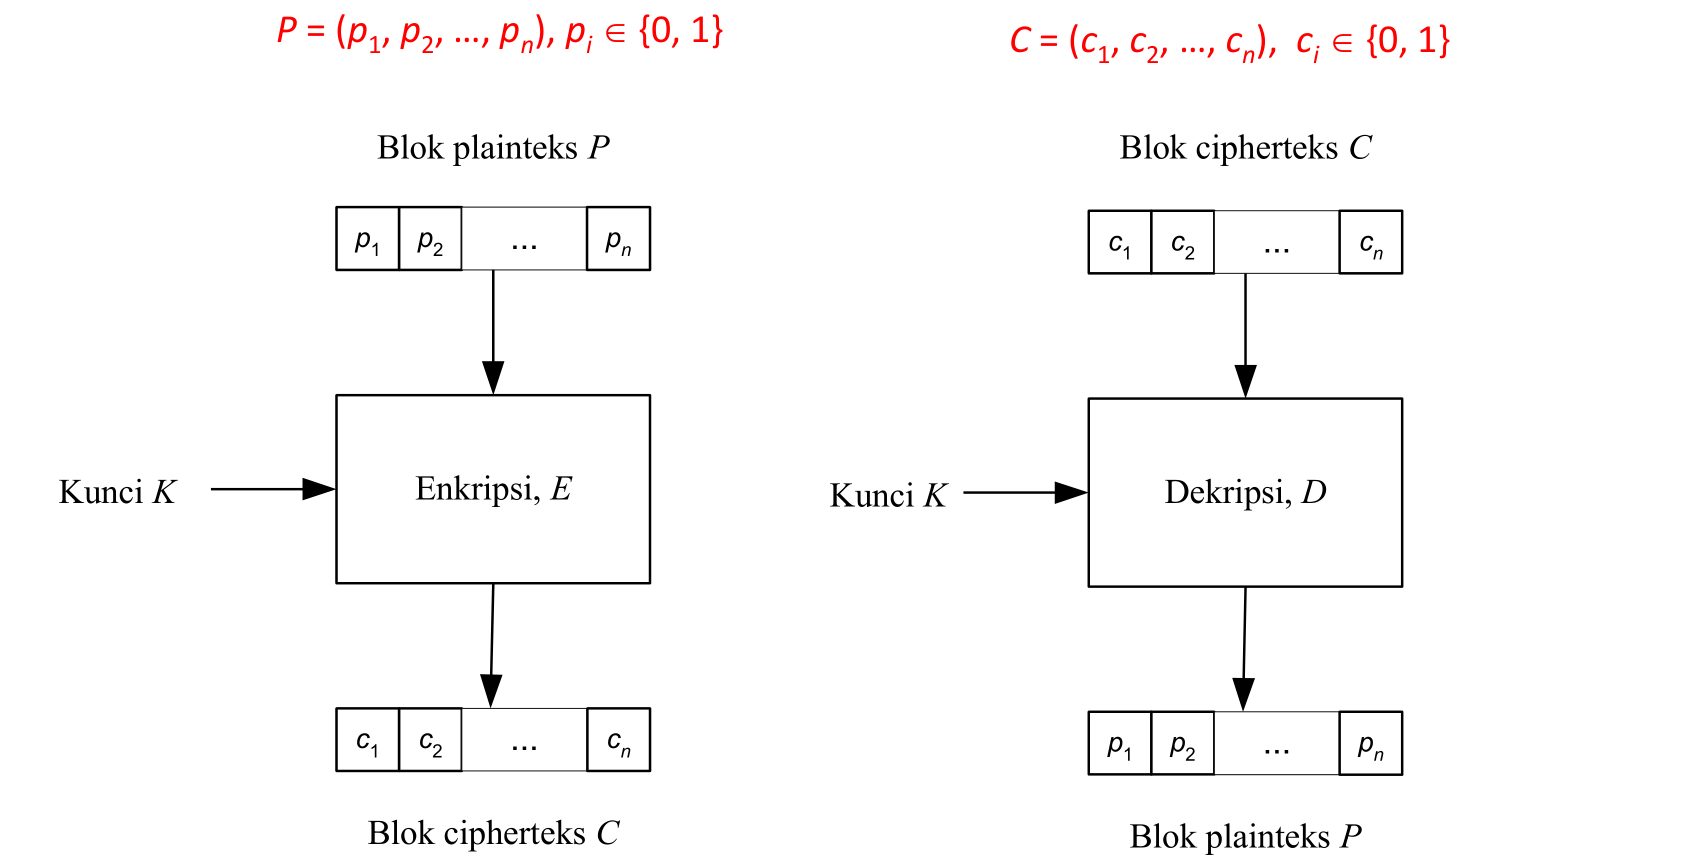
\includegraphics[width=184.80mm,height=238.79mm]{../../images/llm/page_003_img_01.png}%
\end{textblock*}

% deskripsi: Diagram proses dekripsi yang menunjukkan Blok cipherteks C dan Kunci K masuk ke fungsi Dekripsi D untuk menghasilkan kembali Blok plainteks P.
% bbox normalisasi: [0.4900, 0.2200, 0.8000, 0.8900]
\begin{textblock*}{65.10mm}(102.90mm,65.34mm)
\noindent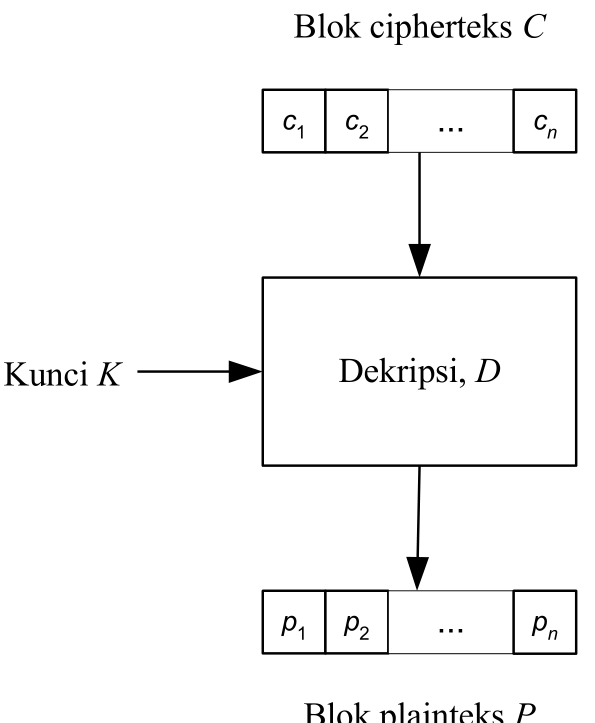
\includegraphics[width=65.10mm,height=198.99mm]{../../images/llm/page_003_img_02.png}%
\end{textblock*}

% bbox perkiraan otomatis: Diagram proses enkripsi yang menunjukkan Blok plainteks P dan Kunci K masuk ke fungsi Enkripsi E untuk menghasilkan Blok cipherteks C.

\end{document}
